\documentclass[13pt]{extreport}
\usepackage[utf8]{vietnam}
%\usepackage{type1cm}
\usepackage[left=3.50cm, right=2.00cm, top=3.50cm, bottom=3.00cm]{geometry}
%\usepackage[left=3.0cm, right=1.50cm, top=3.00cm, bottom=2.50cm]{geometry}
\usepackage{graphicx}
\usepackage{mathrsfs} 
\usepackage{amsfonts}
\usepackage{longtable}
\usepackage[intlimits]{amsmath}
\usepackage{array}
\usepackage{amsxtra,amssymb,latexsym,amscd,amsthm}
\newtheorem{theorem}{\MakeUppercase{K}ết quả}[section]
% khoảng cách dòng 1.5 lines (như trong MS Word)
\renewcommand{\baselinestretch}{1.5}

%——————–
\begin{document}
%tao khung
\newcommand{\Khung}[2]{
\begin{tabular}{|l|}
\hline\rule[-2ex]{0pt}{5.5ex}
\parbox{#1}{#2}\\
\hline
\end{tabular}
}

\Khung{.92\textwidth}{

\begin{center}
\normalsize
\textbf{TRƯỜNG ĐẠI HỌC BÁCH KHOA HÀ NỘI}\\
\normalsize
\textbf{VIỆN TOÁN ỨNG DỤNG VÀ TIN HỌC}\\
\textbf{------------------------------------------------------}\\[0.4cm]

\includegraphics[scale=.8]{logobkdentrang}\\[1.2cm]
\textbf{{\large MÔ HÌNH HÓA DỰA TRÊN CÁ THỂ\\MÔ HÌNH RẦY NÂU HẠI LÚA}}\\[0.3cm]
\textbf{Nghiên cứu ảnh hưởng phân bố không gian của hoa\\thu hút thiên địch rầy lên sự phát triển của rầy nâu}\\[1cm]
\textbf{{\large ĐỒ ÁN TỐT NGHIỆP}}\\[0.2cm]
\textbf{{\large Chuyên ngành: TOÁN TIN}}\\[1cm]
\end{center}
\begin{flushleft}
\hspace{1.5cm} \textbf{ Giáo viên hướng dẫn:\hspace{0.2cm}{ TS. NGUYỄN THỊ NGỌC ANH }}\\[0.2cm]
\hspace{1.5cm} \textbf{ Sinh viên thực hiện:\hspace{0.5cm}{ VŨ THU THẢO}}\\[0.2cm]
\hspace{1.5cm} \textbf{ Lớp:\hspace{4.0cm}{ Toán Tin 2 - K55}}\\
\end{flushleft}

\vspace{1.3cm}
\begin{center}
\textbf{{\large HÀ NỘI - 2015}}\\
\end{center}
 }
\thispagestyle{empty}
\newpage

\tableofcontents
\newpage

%\listoffigures

\newpage
\addcontentsline{toc}{chapter}{{\bf Mở đầu}}
\chapter*{Mở đầu}\
Rầy nâu là một trong những đối tượng dịch hại quan trọng phổ biến nhất trong nhóm rầy hại lúa [1]. Các loại rầy xuất hiện hại lúa theo kiểu chích hút nhựa cây lúa, gây khô và chết cây hoặc truyền virút gây bệnh cho lúa [2]. Rầy gây hại nhẹ làm giảm năng xuất lúa, nặng thì làm khô cây, có thể gây mất trắng thu hoạch [1]. Cách phổ biến nhất người nông dân sử dụng để giải quyết rầy là phun thuốc trừ sâu để diệt rầy. Cách này làm ảnh hưởng đến chất lượng cây lúa, phá vỡ cân bằng môi trường sinh thái và gây tổn hại tới sức khỏe chính người nông dân [10]. Do vậy, thực tế đòi hỏi cần có thêm các giải pháp để diệt rầy đồng thời bảo vệ năng suất lúa gạo một cách hiệu quả, vừa đảm bảo được an ninh lương thực và bền vững môi trường sinh thái. 

Một giải pháp sinh thái được các chuyên gia đề xuất và triển khai gần đây giúp ngăn chặn sự lan truyền rầy nâu và giảm việc sử dụng thuốc trừ sâu là trồng hoa trên các bờ đê dọc theo cánh đồng lúa [9]. Những loại hoa có tác dụng thu hút các loài thiên địch của rầy nâu vào ruộng lúa và những loài thiên địch này sẽ tiêu diệt và làm giảm dân số rầy nâu. Trong đồ án tốt nghiệp này, chúng tôi tập trung nghiên cứu phân bố không gian của các loại hoa dọc theo các bờ đê ảnh hưởng đến quá trình phát triển của rầy nâu và các mối liên hệ giữa các đối tượng trong môi trường sống của rầy nâu: lúa, hoa, rầy nâu, thiên địch, thời gian, không gian, nhiệt độ và vận tốc gió. Vì môi trường sống của rầy nâu có nhiều tính chất phức tạp nên chúng tôi lựa chọn hướng tiếp cận sử dụng mô hình dựa trên cá thể để mô hình hóa hệ thống phức tạp này. Chúng tôi xây dựng một mô hình dựa trên cá thể về rầy nâu, lúa và hoa có tác dụng thu hút thiên địch rầy nâu và sử dụng nó để xây dựng mô phỏng và rút ra kết luận về mối liên hệ giữa phân bố không gian của các loại hoa dọc theo các bờ đê với quá trình phát triển và hại lúa của rầy nâu.

Đồ án được trình bày gồm 5 chương. Trong chương 1, chúng tôi nêu ra và đặt vấn đề xây dựng mô hình đa tác tử của rầy nâu, lúa và hoa thu hút thiên địch rầy. Trong chương 2, chúng tôi giới thiệu một số kiến thức về Mô hình hóa và mô phỏng dựa trên cá thể. Trong chương 3, chúng tôi mô tả và xây dựng mô hình dựa trên cá thể của rầy nâu hại lúa với hai kịch bản phân bố không gian của hoa thu hút thiên địch rầy nâu bằng giao thức ODD. Trong chương 4, chúng tôi trình bày các thí nghiệm mô phỏng và kết quả thu được khi xây dựng chương trình mô phỏng cho mô hình. Chương 5 chúng tôi đưa ra kết luận, nêu lên các kết quả đã đạt đuợc của đề tài và chỉ ra các hướng nghiên cứu tiếp theo.

\indent Mặc dù em đã rất cố gắng hoàn thành đề tài nhưng do hạn chế về kinh nghiệm và kiến thức nên đồ án tốt nghiệp không tránh khỏi nhiều thiếu sót cần được khắc phục. Vì vậy em mong thầy cô và các bạn đóng góp ý kiến để em có thể làm tốt hơn sau này.\\
\indent Cuối cùng, em xin trân trọng cám ơn TS. Nguyễn Thị Ngọc Anh đã tận tình hướng dẫn để em hoàn thành tốt đồ án tốt nghiệp này. Em cũng xin được cảm ơn các thầy cô, anh chị trong nhóm seminar Các mô hình toán học ứng dụng trong hệ điều khiển và hệ sinh thái đã tận tình đóng góp ý kiến để em có thể hoàn thiện đồ án tốt nghiệp này.\\
\begin{flushright}
Hà Nội, 26 tháng 5 năm 2015\\
\textbf{Vũ Thu Thảo}
\end{flushright}

\addcontentsline{toc}{chapter}{{\bf Đặt vấn đề}}
\chapter{Đặt vấn đề}
%lúa - bệnh- rầy- thiên địch- hoa
%đưa ra bài toán- cách tiếp cận giải quyết trong báo cáo
{\indent Lúa là loại cây lương thực lâu năm, được trồng phổ biến ở các nước Châu Á \cite{tltk9}. Nhờ có điều kiện nhiệt độ, độ ẩm, thổ nhưỡng, v.v lí tưởng cho việc phát triển và canh tác cây lúa, từ một nước nhập khẩu gạo, Việt Nam vươn lên trở thành một trong ba nước xuất khẩu lúa gạo lớn nhất trên thế giới hiện nay \cite{tltk10}. Cùng với sự phát triển của cây lúa, các loại dịch bệnh dần xuất hiện, lây lan và gây ảnh hưởng nghiêm trọng đến chất lượng và năng suất lúa gạo. Các dịch bệnh trên lúa thường bị phát tán và lây lan bởi nhiều loại côn trùng, đặc biệt là rầy nâu \cite{tltk9}.}

Rầy nâu hút nhựa và phát tán các loại virus gây bệnh cho lúa như: bệnh lùn sọc đen, bệnh lùn xoắn lá, bệnh sọc gân lá, bệnh Tungro,…\cite{tltk7} - các loại bệnh trên cây lúa mà hiện nay chưa có thuốc đặc trị. Rầy nâu sinh trưởng rất mạnh và tăng trưởng số lượng lớn sau một đợt di chuyển, do đó rầy gây tổn thất rất lớn tới năng suất của lúa vì lúa vừa bị rầy nâu ăn và truyền bệnh. Để ngăn chặn bệnh dịch, nông dân thường chọn giải pháp dùng thuốc trừ sâu. Tuy nhiên, giải pháp này không chỉ có chi phí cao, mà khi người nông dân sử dụng thuốc trừ sâu để làm cho rầy nâu chết thì cũng làm cho các thiên địch của rầy chết theo. Ngoài ra, lượng thuốc trừ sâu thấm xuống đất một thời gian sẽ làm đất bị ô nhiễm và dẫn đến môi trường xung quanh cũng bị ô nhiễm. Trong những năm gần đây, một giải pháp sinh thái được đề xuất và áp dụng tại vùng Đồng bằng Sông Cửu Long để giúp ngăn chặn sự lan truyền rầy nâu là trồng hoa xung quanh bờ đê của ruộng lúa (Hình 1.1). Những loại hoa này có tác dụng thu hút các loài thiên địch của rầy nâu vào ruộng lúa và những loài thiên địch này sẽ tiêu diệt và ngăn sự tăng trưởng và lây lan rầy nâu trên ruộng \cite{tltk8}.

Trong đồ án tốt nghiệp, chúng tôi tập trung trình bày nghiên cứu phân bố không gian của các loài hoa trên ruộng ảnh hưởng đến quá trình phát triển của rầy nâu. Chúng tôi tìm các mối liên hệ giữa các đối tượng trong môi trường sống của rầy nâu: lúa, hoa, thiên địch, thời gian, không gian, nhiệt độ và hướng, vận tốc gió. Vì sự phát triển của rầy nâu bị ảnh hưởng bởi nhiều nhân tố môi trường phức tạp, chúng tôi lựa chọn sử dụng mô hình dựa trên cá thể để mô hình hóa hệ thống phức tạp này. 

Việc mô hình hóa mô phỏng sự phát triển của rầy nâu có lợi thế là mô phỏng có thể lặp lại và từ đó con người có thể kiểm soát được các tình huống với các điều kiện mô phỏng khác nhau nhiều lần mà không tốn kém chi phí lớn. Mô phỏng giúp quan sát sự phát triển của cá thể và dự đoán được nhiều đặc trưng mới của quần thể \cite{tltk12}. Quần thể rầy được mô phỏng trong các điều kiện môi trường thời tiết như thực tế, qua đó, chúng tôi đưa ra đánh giá và đề xuất một số giải pháp ứng dụng và chính sách để hạn chế sự phát triển loài rầy \cite{tltk13}. Trong đồ án tốt nghiệp này, chúng tôi sử dụng GAMA - một công cụ cung cấp môi trường mô hình hóa mô phỏng - để xây dựng không gian mô hình mô phỏng dựa trên cá thể.

Trước khi đi vào xây dựng mô hình, chúng tôi sẽ giới thiệu một số khái niệm mở đầu và tổng quan về Mô hình hóa và mô phỏng dựa trên cá thể - hướng tiếp cận mô hình hóa được tôi sử dụng để thực hiện nghiên cứu trong đồ án này. Chi tiết nội dung được trình bày trong Chương 2.
\begin{figure}
\begin{center}
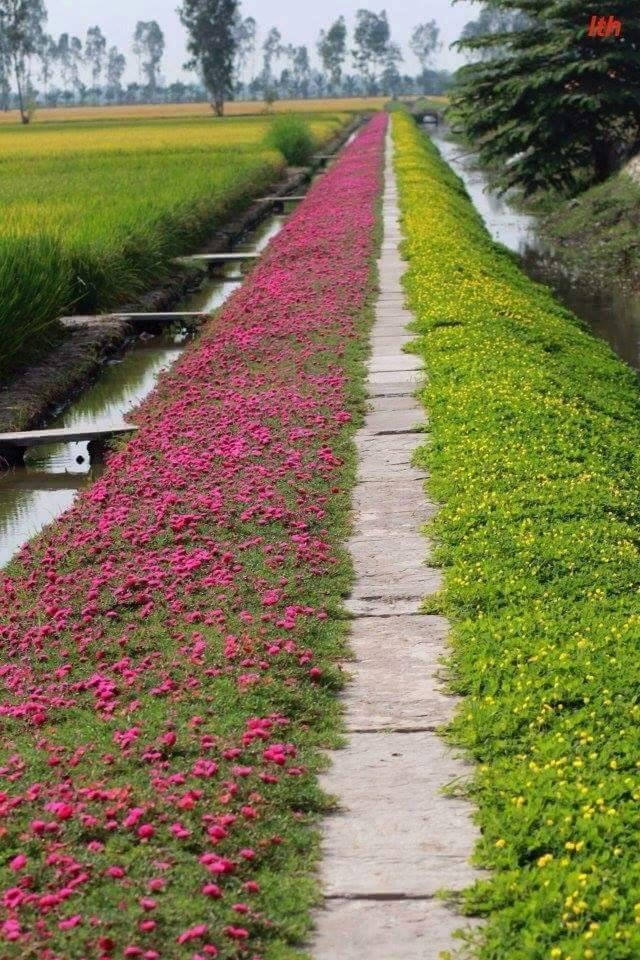
\includegraphics[scale=0.5]{photo1}
\end{center}
\caption{\textit{ Hoa được trồng xung quanh ruộng lúa ở An Giang}}
\end{figure}

\newpage
\chapter{Giới thiệu về mô hình hóa và mô phỏng dựa trên cá thể}

\section{Mô hình hóa và mô phỏng dựa trên cá thể}
Mục đích của chương này là giới thiệu về mô hình hóa và mô phỏng dựa trên cá thể. Từ một số khái niệm ban đầu về mô hình và mô hình hóa, ta hiểu và trả lời được những câu hỏi cơ bản:
\begin{itemize}
\item Mô hình và mô hình hóa là gì. Tại sao người ta cần xây dựng mô hình?
\item Chu trình phát triển mô hình, quá trình tương tác giữa việc thiết kế, cài đặt, phân tích mô hình và sử dụng nó để giải quyết các bài toán phức tạp trong thực tế.
\item Mô hình dựa trên cá thể là gì và nó có gì khác so với các loại mô hình khác. Tại sao và khi nào ta cần sử dụng mô hình dựa trên cá thể?
\end{itemize}

\subsection{Mô hình là gì?}
\indent {Mô hình là một biểu diễn của một hệ thống thực tế nhằm hướng tới giải quyết một vấn đề nhất định [7].} Chúng ta xây dựng và sử dụng các mô hình để giải quyết hay trả lời những câu hỏi về một hệ hay một lớp các hệ thống. Trong khoa học, người ta thường muốn hiểu rõ cách mọi thứ vận hành và hoạt động, giải thích những đặc trưng quan sát được và dự đoán hành vi của hệ nếu có sự thay đổi về yếu tố nào đó. Các hệ thống trong thực tế thường rất phức tạp hoặc mất thời gian quá lâu để ta có thể thực hiện thử nghiệm phân tích. Yêu cầu thực tế đòi hỏi ta cần mô hình hóa, hay xây dựng một biểu diễn đơn giản hơn của hệ thống. Việc này thường thực hiện bởi các phương trình toán học và chương trình máy tính, từ đó ta có thể điều khiển và thử nghiệm mô hình đã xây dựng.

%Ta có thể biểu diễn một hệ thống thực (ví dụ: một thành phố, một khu rừng...) theo nhiều cách. Nhưng làm thế nào để ta quyết định giữ hay bỏ qua yếu tố nào của hệ thống thực trong mô hình của mình? Câu trả lời phụ thuộc vào mục đích lập mô hình.

\subsection{Chu trình phát triển mô hình}
\indent Để mô hình hóa một cách khoa học một mô hình, người làm mô hình cần lập mô hình theo một quy trình có hệ thống và sau đó sử dụng các công thức toán học và chương trình máy tính để kiểm tra. Việc này giúp xác định tính chặt chẽ và chính xác kết quả của các giả thiết được đưa ra khi ta lập mô hình. Mô hình ban đầu được đưa ra có thể quá đơn giản hoặc quá phức tạp, hay có thể câu hỏi được đặt ra ban đầu cho mô hình là chưa hợp lí mà ta không phát hiện ra. Vì vậy, chu trình phát triển mô hình là một đòi hỏi cần thiết.

Chu trình phát triển mô hình dựa trên cá thể bao gồm 6 bước \cite{grim05}:

\textbf{Bước 1: Người lập mô hình phải xác định các câu hỏi mà mô hình phải giải quyết}

Giải quyết  một bài toán có nghĩa là chúng ta phải trả lời các câu hỏi mà bài toán đặt ra. Mục đích của viêc lập mô hình chính là giải quyết một bài toán nào đó trong hệ thống thực bằng việc biểu diễn các khía cạnh của hệ thống thực. Chính vì vậy mà người lập mô hình phải xác định câu hỏi mà mô hình phải giải quyết.

Nhiệm vụ này tương tự như việc đọc lại bài toán, nó sẽ giúp cho người lập mô hình hiểu về hệ thống. Để giải quyết bài toán, trước hết người lập mô hình phải xem xét mọi thành phần và tiến trình đã biết của hệ thống thật và quyết định xem chúng có cần thiết cho việc giải quyết bài toán không. Nhờ vậy, mô hình được xấy dựng sẽ không quá phức tạp, nhưng vẫn đủ để giải quyết bài toán.

\textbf{Bước 2: Người lập mô hình phải thiết lập các giả thuyết cho các quá trình và cấu trúc cơ bản}

Cấu trúc cơ bản của mô hình dựa trên cá thể là một tập hợp các cá thể độc lập. Các quá trình là nguyên nhân làm thay đổi biến trạng thái và các tham số được sử dụng trong mô hình. Cấu trúc và quá trình cơ bản là hai thành phần cấu tạo nên mô hình. Việc xây dựng mô hình là làm việc với các giả thuyết, do đó, người lập mô hình cần phải thiết lập các giả thuyết cho các quá trình và cấu trúc cơ bản.

Những giả thuyết này đầu tiên được phản ánh trong những hiểu biết sơ bộ về hệ thống, mà trong thực tế là những khái niệm ban đầu về mô hình. Trong mỗi khái niệm, chúng ta giải thuyết cái gì là quan trọng, cái gì có thể bắt đầu chu kì của mô hình.

Có hai nguồn chính để xây dựng các giả thuyết: lý thuyết và kinh nghiệm. Lý thuyết chính là cơ sở chúng ta nhận thức hệ thống. Kinh nghiệm được định hình bởi lý thuyết hoặc bằng việc chúng ta sử dụng hệ thống.

\textbf{Bước 3: Người lập mô hình phải xác định phạm vi, các biến trạng thái, các quá trình và các tham số cho mô hình}

Người lập mô hình phải chọn các biến cần thiết để mô tả được trạng thái của hệ thống. Các biến này được gọi là các biến trạng thái và sự biến đổi của các biến trạng thái phụ thuộc vào các quá trình cơ bản. Để mô tả một cá thể và một mô hình hoàn chỉnh, người lập mô hình phải sử dụng hàng nghìn biến trạng thái. Nhưng đây không phải là mục đích chính. Ta chỉ cần xác định những thuộc tính của cá thể là cần thiết cho câu hỏi mà ta đang cố gắng đi tìm câu trả lời.

Nếu danh sách biến trạng thái quá dài, nó sẽ gây khó khăn cho việc phát triển mô hình. Do đó, ta cần phải giới hạn danh sách các biến trạng thái bằng cách loại bỏ các biến không cần thiết trong mô hình.

Trong mô hình, các tham số được sử dụng trong các biểu diễn và quy tắc. Để biểu diễn các quá trình và cấu trúc cơ bản, các tham số có thể là hằng số không đổi hoặc biến đổi.

Việc chọn biến, các tham số và các biểu thức biểu diễn, các quy tắc sử dụng gắn liền với việc chọn phạm vi mô hình. Phạm vi gồm hai khía cạnh:
\begin{itemize}
\item Chi tiết: Đơn vị thời gian hoặc đơn vị không gian chúng ta dự định xét đến.
\item Khái quát: Thới gian tổng hoặc vùng không gian bao phủ mô hình.
\end{itemize}
Để hiểu rõ một mô hình dựa trên cá thể, chúng ta phải biết các quá trình nào thuộc về môi trường và các quá trình nào là của cá thể được xây dựng trong mô hình. Sự thực hiện các quá trình cũng được xét ở hai mức. Ở mức thấp, các quá trình được thực hiện bởi các thực thể. Ở mức cao, các quá trình được thực hiện bởi con người.

\textbf{Bước 4: Lập mô hình}

Ở bước này, người lập mô hình sẽ làm hai công việc chính: thiết kế và viết chương trình. Trước khi thực hiện, người lập mô hình phải lên kế hoạch lập mô hình. Điều quan trọng là chương trình có cho phép người lập mô hình quan sát và điều khiển thí nghiệm trên tất cả các thành phần của mô hình dựa trên cá thể hay không. Chương trình không chỉ thực hiện mô hình, nó còn phải cung cấp được một phòng thí nghiệm ảo cho các thí nghiệm trên mô hình.

\textbf{Bước 5: Phân tích đánh giá mô hình}

Phân tích mô hình nghĩa là ta phải so sánh và đánh giá nó với các phiên bản trước đó. Cần phải xác định một tiêu chuẩn chung để so sánh các phiên bản của mô hình. Kiểm tra mô hình là việc ước lượng độ tin cậy của các kết quả thu được.

Mục đích của phân tích và kiểm tra mô hình là để cải thiện mô hình. Cải thiện một mô hình bao gồm các việc: đơn giản hóa mô hình bằng cách loại bỏ các nhân tố chung chung không cần thiết; thiết lập các giải pháp khi các nhân tố chung chung được miêu tả không đúng cách; chỉnh sửa các tiến trình hoặc cấu trúc; chỉnh sửa bản sao các quan sát tốt hơn, làm mô hình dễ hiểu hơn; đưa ra nhiều dự đoán hơn.

Tuy nhiên ta không thể chỉ dừng ở bước này. Điều chúng ta cần là một quy tắc dừng để đánh giá mô hình đã xây dựng là đủ tốt. Quy tắc này phải xác định từ khi bắt đầu vì nó ảnh hưởng chính tới việc thiết kế mô hình. Quy tắc dừng giống như các thành phần chính của mô hình, nó có thể thay đổi trong suất quá trình phát triển mô hình. Trong thực tế, hầu hết quy tắc dừng quan trọng là các ràng buộc về thời gian và tài nguyên.

\textbf{Bước 6: Báo cáo mô hình}

Người lập mô hình phải báo cáo về mô hình và kết quả của nó cho cộng đồng khoa học hoặc các nhà quản lí có dự định sử dụng mô hình. Nội dung của báo cáo là các kết quả quan sát, kết quả thí nghiệm, các phát hiện và các tri thức thu đươc từ mô hình.

%ABM là mô hình trong đó các cá thể (hay các loài) được mô tả như các thực thể duy nhất và độc lập, tương tác với nhau và với môi trường xung quanh. Các loài do đó sẽ có các hành vi thích ứng: Chúng có thể điều chỉnh hành vi của mình, của loài khác hay của môi trường. Sử dụng mô hình ABM cho chúng ta khả năng hướng tới vấn đề sự nổi bật cần quan tâm đến khi nghiên cứu mô hình: hệ động lực xét tới các thành phần cá thể của hệ tương tác với nhau và với môi trường như thế nào. Từ đó, ta có thể nghiên cứu các câu hỏi về các hành vi của hệ xuất phát từ, hay có liên hệ thế nào với các đặc trưng và hành vi của các cá thể thành phần.
%Thông thường, một số nhà khoa học chỉ nghiên cứu về các hệ động lực, mô hình hóa và xét các sự thay đổi của toàn hệ dựa vào hướng tiếp cận phương trình đạo hàm riêng. Một số nhà khoa học khác chỉ nghiên cứu đến các loài như việc các cây cối, loài vật, con người...thay đổi và thích ứng như thế nào với các điều kiện bên ngoài. Mô hình hóa dựa trên cá thể quan tâm tới cả hai mức này và cả tương tác giữa chúng: các cá thể sẽ thay đổi ra sao nếu hệ thay đổi và hệ động lực thay đổi thế nào nếu các cá thể của nó thay đổi. Mô hình hóa dựa trên cá thể tập trung mô phỏng hành vi của các cá thể, đồng thời cho ta quan sát và hiểu hành vi của hệ bị ảnh hưởng bởi cá thể trong hệ. 
%o phần lớn các giả thiết mô hình chỉ là thử nghiệm, các mô hình được xây dựng cần phải được kiểm tra lại: ta cần chạy và phân tích các giả thuyết được đưa ra. Với nhiều mô hình phức tạp trong khoa học và thực tế, ta cần thực hiện các chương trình mô phỏng và lặp lại nhiều lần để có thể đưa ra kết luận chặt chẽ cho các giả thiết được đưa ra.
\subsection{Mô hình hóa dựa trên cá thể}
\indent Trước đây, sự phức tạp của một mô hình khoa học thường bị giới hạn bởi khả năng xử lí toán học: khi các phương trình trong giải tích là cách duy nhất để mô hình hóa một hệ, ta phải đảm bảo mô hình đủ đơn giản để có thể giải được, vì thể, các mô hình có thể mô hình hóa bị giới hạn chỉ là những vấn đề khá đơn giản.

Nhờ khả năng mô phỏng của máy tính, các giới hạn của việc xử lí toán học dần được gỡ bỏ. Hình 2.1 trình bày một số cách đã được sử dụng để tiếp cận xây dựng một mô hình thực tế. Ta có thể tiếp cận nhiều mô hình phức tạp hơn, biểu diễn nhiều đặc trưng thực tế của mô hình hơn. Mô hình hóa dựa trên cá thể là một trong số đó. Mô hình hóa dựa trên cá thể biểu diễn từng thành phần cá thể của mô hình và hành vi của chúng. Thay vì mô tả cả mô hình  với các biến trạng thái của cả hệ, ta mô hình hóa từng cá thể riêng biệt của hệ.

Mô hình hóa dựa trên cá thể (Individual-based model, viết tắt là \textit{IBM}) là phương pháp mô hình trong đó các cá thể (hay các loài) được mô tả như các thực thể duy nhất và độc lập, tương tác với nhau và tương tác địa phương với môi trường xung quanh. Các cá thể (hay loài) có thể là vi sinh vật, con người, các tòa nhà hay bất kì một thực thể nào có mục tiêu nhất định. Tính duy nhất tức là các cá thể thường khác nhau về các đặc trưng như kích cỡ, vị trí, năng lượng. Tương tác địa phương nghĩa là các cá thể không chỉ tương tác với tất cả các cá thể khác mà chỉ có tương tác trong phạm vi "hàng xóm" của chúng, về mặt không gian địa lý hay hệ thống "mạng" nào đó. Độc lập nhấn mạnh mục tiêu riêng và khả năng hoạt động độc lập của mỗi cá thể. Các loài do đó sẽ có các hành vi thích ứng: Chúng có thể điều chỉnh hành vi của mình, của loài khác hay của môi trường. 

Sử dụng mô hình dựa trên cá thể cho chúng ta khả năng hướng tới vấn đề sự nổi bật cần quan tâm đến khi nghiên cứu mô hình: hệ động lực xét tới các thành phần cá thể của hệ tương tác với nhau và với môi trường như thế nào. Từ đó, ta có thể nghiên cứu các câu hỏi về các hành vi của hệ xuất phát từ đâu, hay có liên hệ thế nào với các đặc trưng và hành vi của các cá thể thành phần.

\begin{figure}
\begin{center}
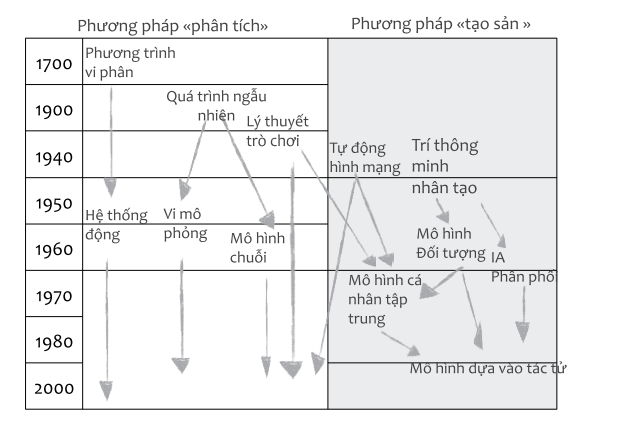
\includegraphics[scale=0.7]{huongmh}
\end{center}
\caption{\textit{ Các hướng tiếp cận phân tích một mô hình [3]}}
\end{figure}

Mô hình hóa dựa trên cá thể rất hữu ích cho các vấn đề quan tâm đến sự nổi bật của mô hình bởi nó là phương pháp mô hình hóa có thể xem xét được mô hình đa mức. Thông thường, một số nhà khoa học chỉ nghiên cứu về các hệ động lực, mô hình hóa và xét các sự thay đổi của toàn hệ dựa vào hướng tiếp cận phương trình. Một số nhà khoa học khác chỉ nghiên cứu đến các loài như việc các cây cối, loài vật, con người... thay đổi và thích ứng như thế nào với các điều kiện bên ngoài. Mô hình hóa dựa trên cá thể quan tâm tới cả hai mức này và cả tương tác giữa chúng: các cá thể sẽ thay đổi ra sao nếu hệ thay đổi và hệ động lực thay đổi thế nào nếu các cá thể của nó thay đổi. Mô hình hóa dựa trên cá thể tập trung mô phỏng hành vi của các cá thể, đồng thời cho ta quan sát và hiểu hành vi của hệ bị ảnh hưởng bởi cá thể trong hệ. 

Tuy vậy, khả năng mô hình hóa các mô hình phức tạp và đa mức của mô hình dựa trên cá thể yêu cầu người xây dựng mô hình cần trang bị thêm nhiều kĩ năng mới. Cách tiếp cận xây dựng mô hình trước đây yêu cầu cao về các kĩ năng toán học, đặc biệt là giải tích vi phân và thống kê. Mô hình hóa dựa trên cá thể không đòi hỏi sâu về kiến thức toán học đó mà đòi hỏi người làm mô hình nghĩ và mô tả mô hình theo một "ngôn ngữ" mới với một chuẩn các khái niệm mới (ví dụ như sự nổi bật, hành vi thích nghi, tương tác, cảm giác) để mô tả các thành phần chính yếu khi sử dụng. Thêm vào đó, người làm mô hình cần có kĩ năng xây dựng chương trình trên máy tính để quan sát, kiểm tra, điều khiển và phân tích mô hình của mình vì xây dựng chương trình cho mô hình dựa trên cá thể thường phức tạp hơn nhiều so với các loại mô hình khác. Hơn thế nữa, mô hình hóa dựa trên cá thể đòi hỏi một chiến lược rõ ràng cho việc thiết kế và phân tích mô hình. Tuy ta không có giới hạn về độ phức tạp cho một mô hình được mô phỏng, nhưng một mô hình quá phức tạp sẽ khiến việc tham số hóa, kiểm tra và phân tích trỏ nên rất khó khăn. Người làm mô hình cần xác định các thực thể, biến trạng thái, các tiến trình nào là cần thiết cho mô hình xây dựng, từ đó giúp phân tích và thu nhận các kiến thức từ mô hình thực tế. 


\subsection{Kết luận}

Trong phần 2.1, chúng tôi đã giới thiệu và trình bày một số khái niệm cơ bản ban đầu về mô hình, chu trình phát triển mô hình và mô hình hóa dựa trên cá thể. Mô hình hóa dựa trên cá thể yêu cầu cần có những công cụ xây dựng và thực hiện các thí nghiệm mô phỏng thích hợp cho người làm mô hình. Trong phần tiếp theo, chúng tôi sẽ giới thiệu về GAMA - một trong những phần mềm thường được người làm mô hình dựa trên cá thể sử dụng, cũng là phần mềm mà chúng tôi sử dụng để thực hiện chương trình mô phỏng trong đồ án này.

\section{GAMA - một phần mềm mô phỏng sử dụng để mô hình hóa dựa trên cá thể}

\subsection{Tổng quát về GAMA}
\indent GAMA là một nền tảng cung cấp môi trường mô hình hóa và mô phỏng hoàn chỉnh để xây dựng không gian mô phỏng dựa trên cá thể. Phần mềm được phát triển bởi một nhóm nghiên cứu người Pháp, Việt Nam dưới sự bảo trợ của IRD/UPMC International Research Unit UMMISCO từ năm 2007 \cite{tltk11}.

Được phát triển như một "plugin" của Eclipse, GAMA có giao diện sử dụng tương tự với Eclipse. Đặc biệt là giao diện Editor, Views và Perspective. Người dùng sử dụng Views và Editors và các nhãn để hiển thị thông tin (trong trường hợp xem) và chỉnh sửa các tập tin (trong trường hợp chỉnh sửa). Ví dụ, GAMA Navigator cho phép hiển thị các thư viện dự án. Perspective là một công cụ trực quan để tổ chức một tập các theo dõi và chỉnh sửa.

GAMA là một nền tảng mô phỏng nhằm hướng tới các lĩnh vực chuyên môn, nhà mô hình. Do dựa trên nền tảng Java nên GAMA có thể chạy trên 3 nền hệ điều hành phổ biến hiện nay là Windows, Mac OS, Linux. Thư viện mẫu có sẵn của GAMA rất phong phú. Dung lượng bộ cài đặt nhỏ gọn, dễ cài đặt làm cho nó ngày càng được sử dụng phổ biến. Thêm vào đó, qua các phiên bản, giao diện GAMA luôn được cải tiến để giao diện thân thiện hơn với người dùng. 

\subsection{Các tính năng chính của GAMA}
\indent Các tính năng nổi nổi trội của GAMA so với các phần mềm mô phỏng khác (Netlogo, Repast, Cormas,...) bao gồm:
\begin{itemize}
\item Có khả năng sử dụng dữ liệu phức hợp dữ liệu địa lý GIS như một môi trường cho các cá thể;
\item Có khả năng xử lý một lượng rất lớn (hỗn hợp) các cá thể;
\item Có khả năng cung cấp nền tảng cho thí nghiệm điều khiển tự động (bằng cách tự động chỉnh nhiều tham số, ghi lại các thống kê...vv);
\item Có khả năng định nghĩa các mô hình đa mức
\item Dễ dàng sử dụng ngay với những nhà khoa học không thuộc chuyên ngành máy tính. Tương tác với các cá thể trong quá trình chạy giả lập.
Ngoài ra GAMA cũng cung cấp:
\item Cung cấp một ngôn ngữ mô hình hóa hoàn chỉnh dựa trên XML là GAML để mô hình hóa các cá thể và môi trường
\item Cung cấp thư viện lớn và khả năng mở rộng cao (sự di chuyển của cá thể, giao tiếp, các hàm toán học, đồ thị,...)
\item Hệ thống vẽ đồ thị mạnh mẽ, linh hoạt.
\item Cung cấp một tập hợp hoàn chỉnh các công cụ xử lý hàng loạt. GAMA Cho phép sự thăm dò thông minh, có hệ thống đối với tập các tham số của mô hình.
\end{itemize}

\subsection{Lập trình và sử dụng GAMA}
\subsubsection*{Giao diện soạn thảo GAMA}
\begin{figure}
\begin{center}
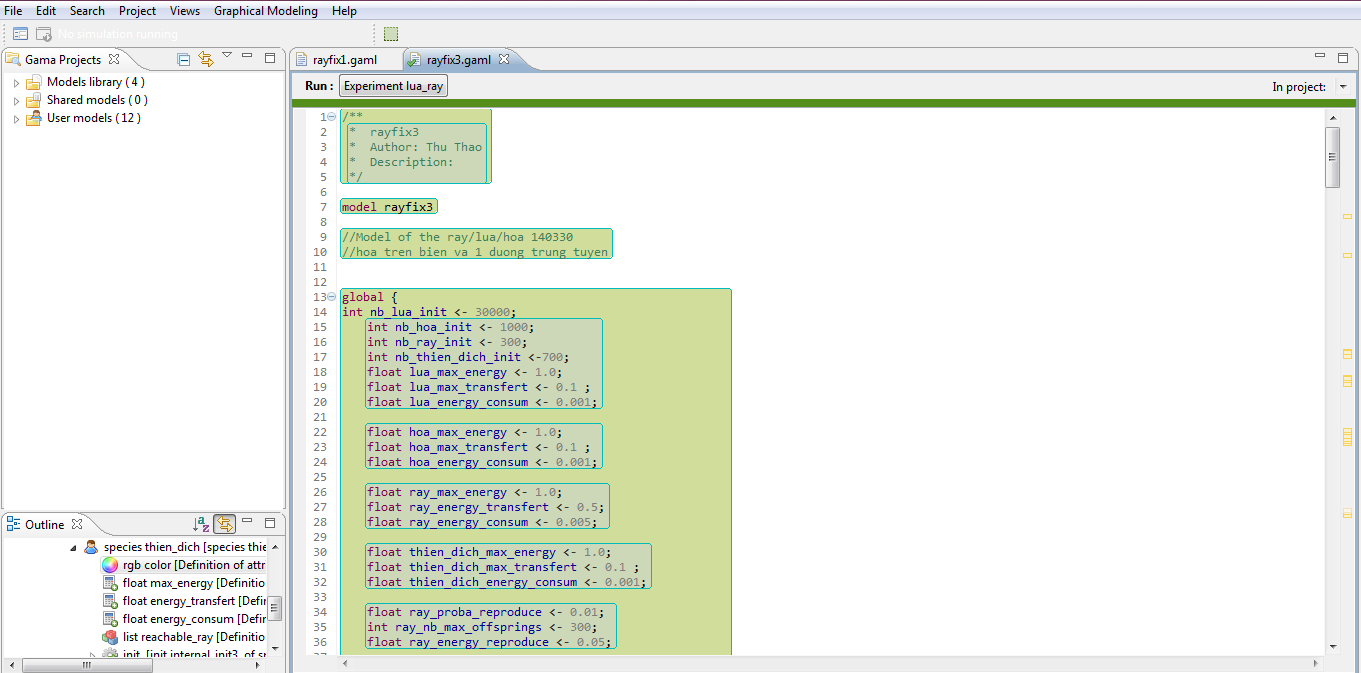
\includegraphics[scale=0.4]{khung_gama}
\end{center}
\caption{\textit{ Giao diện soan thảo GAMA}}
\end{figure}

Giao diện soạn thảo GAMA được chia làm 3 phần  chính (Hình 2.2):

a.  Cửa  sổ duyệt  các mô hình:  Thư  viện  các mô hình  có sẵn  trong GAMA và các mô hình được tạo bởi người dùng sẽ hiển thị ở đây. Thư viện có sẵn chứa rất  nhiều các mô hình khác nhau  được phân loại và để trong  các thư  mục con.

b.  Khung  soạn thảo:  hiển thị  các dòng lệnh của mô hình  đang  được soạn thảo.  Một mô hình được chia làm 4 phần: 

–  Khai  báo toàn  cục (Global):  khai  báo các biến,  các tham  số và các lệnh có tác  dụng trên  toàn  mô hình.

–  Môi trường  (Environment): khai báo các biến, thể  hiện hành động có tác dụng cho môi trường  trong  mô hình.  Môi trường này có thể được tạo trực tiếp hoặc ta có thể lấy từ môi trường ngoài như dữ liệu GIS, tập  tin  ảnh...

–  Thực thể (Entities): khởi tạo các cá thể, các biến và các hành vi của loài.

–  Thử nghiệm (Experiment): Bối cảnh thực hiện mô phỏng, xác định các điều kiện cho đầu  vào và đầu  ra.

c.  Cửa  sổ phác  thảo:  tóm  tắt cho người sử dụng  biết  các biến,  các hành  động...được  khai báo trong  khung  soạn thảo.

\subsubsection*{Giao diện chạy mô phỏng GAMA}
\begin{figure}
\begin{center}
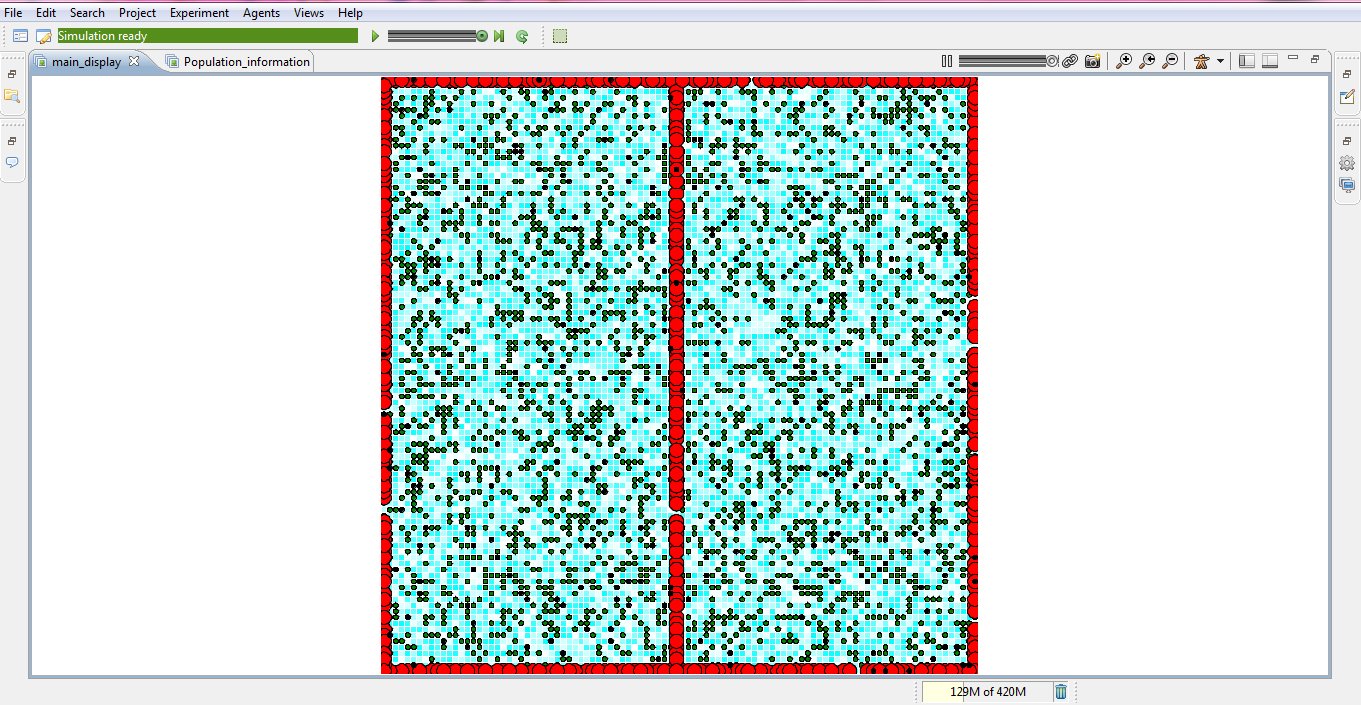
\includegraphics[scale=0.4]{gama}
\end{center}
\caption{\textit{ Giao diện chạy mô phỏng GAMA}}
\end{figure}

Giao diện chạy mô phỏng  GAMA gồm 3 phần (Hình 2.3):

a.  Cửa sổ duyệt  các mô hình.

b.  Khung  hiển thị kết quả chạy: hiển thị kết quả chạy bằng hình ảnh.
Cung  cấp kết quả chạy mô phỏng  một  cách trực  quan.

c.  Cửa  sổ phác  thảo:  tóm  tắt cho người sử dụng  biết  các biến,  các hành  động... được  khai báo trong  khung  soạn thảo

\subsection{Kết luận}
\indent Trong phần 2.2, chúng tôi đã giới thiệu tổng quan về phần mềm mô phỏng GAMA, các tính năng chính và cách lập trình sử dụng GAMA. Mô hình dựa trên cá thể của rầy nâu, lúa và hoa thu hút thiên địch rầy mà chúng tôi nghiên cứu xây dựng là một mô hình cần xét tới một số lượng lớn cá thể của mỗi loài. Hơn nữa, các loài trong mô hình cũng có rất nhiều các yếu tố môi trường ảnh hưởng và tương tác phức tạp. Với các thế mạnh về tính năng đã nêu trong phần 2.2.2, chúng tôi lựa chọn GAMA là công cụ để xây dựng chương trình mô phỏng cho đồ án. Trong phần tiếp theo, chúng tôi sẽ giới thiệu về ODD - một giao thức để mô tả mô hình dựa trên cá thể mà chúng tôi sử dụng để mô tả và xây dựng mô hình chúng tôi nghiên cứu trong đồ án này.

\section{Giao thức ODD mô tả mô hình dựa trên cá thể}
\subsection{Giới thiệu về giao thức ODD}
\indent Các mô hình mô phỏng các cá thể trong sinh thái học hoặc khái quát hơn là "đa tác tử" đã trở thành công cụ được sử dụng rộng rãi không chỉ trong sinh thái học mà còn trong nhiều lĩnh vực khác như vật lý, kinh tế, địa lý.... Mô hình dựa trên cá thể cho phép các nhà nghiên cứu tìm hiểu các thuộc tính nổi bật từ các hành vi thích nghi của các cá thể cũng như làm thế nào hệ thống ảnh hưởng đến các cá thể. Mô hình dựa trên cá thể rất quan trọng cho cả lý thuyết và quản lí vì nó là mô hình có thể cho phép nhà nghiên cứu xét đến các khía cạnh thường bị bỏ qua trong các mô hình dựa trên phương trình như; sự khác biệt giũa các cá thể, sự tương tác cục bộ, vòng đời và hành vi thích nghi của cá thể.

Có hai vấn đề gặp phải khi mô tả mô hình dựa trên cá thể:
\begin{itemize}
\item[(i)]Không có giao thức chuẩn để mô tả.
\item[(ii)]Mô hình dựa trên cá thể thường được mô tả một cách khái quát mà không có những giải thích rõ ràng cho các biểu thức, quy tắc và lịch trình được sử dụng trong mô hình.
\end{itemize}

Từ yêu cầu để giải quyết các vấn đề trên, giao thức ODD (Overview, Design concepts and Details- viết tắt là \textit{ODD}) được đưa ra bởi Volker Grimm mô tả mô hình dựa trên cá thể
vào năm 2006 và được điều chỉnh lại vào năm 2010 \cite{Grimm2006115, Grimm20102760}. Giao thức ODD giúp mô hình được mô tả theo một cấu trúc chuẩn với các khái niệm, quy tắc, các phương trình, các tham số và các biến trong mô hình được giải thích rõ ràng. Giao thức ODD cũng đã được công nhận rộng rãi bởi hầu hết những nhà nghiên cứu mô hình dựa trên cá thể.

\subsection{Các thành phần của giao thức ODD}
\indent Khái quát các thành phần của giao thức ODD được trình bày như trong Bảng 2.1

\begin{table}
\begin{tabular}{|c l|c|}
\hline
\textit{Khái quát} & \textit{Mục đích} \\  
{} & \textit{Các thực thể, biến trạng thái và phạm vi} \\ 
{} & \textit{Tiến trình và kế hoạch} \\ 
\cline{1-2}
\textit{Các khái niệm nền tảng} & \textit{Các khái niệm nền tảng} \\ 
\cline{1-2}
\textit{Chi tiết} & \textit{Khởi tạo} \\ 
{} & \textit{Dữ liệu đầu vào} \\ 
{}& \textit{Mô hình con} \\ 
\hline
\end{tabular} 
\caption{\textit{Các thành phần chính của giao thức ODD}}
\end{table}

\subsubsection{Mục đích của mô hình}
\indent Mỗi mô hình đều được bắt đầu từ một bài toán, một vấn đề hoặc một giả thuyết. Do vậy, giao thức ODD bắt đầu với một tóm tắt ngắn gọn về mục tiêu mà mô hình phát triển. Nếu không biết mục đích của mô hình thì người đọc sẽ không hiểu tại sao khía cạnh này lại được mô tả trong mô hình mà không phải là khía cạnh khác. Thông thường, mục đích của một mô hình được trình bày ở phần đầu mô hình. Mục đích của mô hình không cho biết mô hình hoạt động thế nào, nó chỉ cho biết cái gì được mô hình sử dụng và khía  cạnh nào của mô hình được mô tả tiếp. Ngoài ra, mục đích của một mô hình còn cho biết tại sao người lập mô hình cần xây dựng mô hình phức tạp, điều gì trong mô hình là tổng quát, điều gì cần chi tiết và người lập mô hình dự định làm gì với mô hình của họ.
\subsubsection{Các thực thể, biến trạng thái và phạm vi mô hình}
\textit{\textbf{\indent Thực thể}}: là đối tượng hoặc các tác nhân có hành vi riêng biệt, có thể tương tác với các đối tượng hoặc tác nhân khác và chịu ảnh hưởng của các nhân tố của môi trường bên ngoài.\\
Hầu hết các mô hình dựa trên cá thể gồm có các loại thực thể sau: cá thể, đơn vị không gian, môi trường, các nhóm cá thể.

\textit{\textbf{Các cá thể}}: Một mô hình có thể có nhiều loại cá thể và trong từng loại cá thể  cũng có những loại không giống nhau.

\textit{\textbf{Đơn vị không gian:}} vùng không gian nhỏ nhất được xét trong mô hình. Đơn vị không gian thường dùng để biểu diễn các điều kiện môi trường.

\textit{\textbf{Môi trường:}} là thực thể ảnh hưởng đến các hành vi và sự biến đổi của tất cả cá thể.

\textit{\textbf{Tập thể:}} là nhóm các cá thể, các nhóm này có thể có hành vi riêng. Một tập thể thường biểu thị đặc điểm bằng một danh sách các tác nhân của nó và các hành động cụ thể chỉ được thực hiện bởi tập thể.

\textit{\textbf{Biến trạng thái:}} là các biến để phân biệt thưc thể này với thực thể khác và nó cũng là dấu hiệu cho biết sự thay đổi của thực thể theo thời gian. Biến trạng thái có thể là biến giới tính, tuổi, màu sắc...

\textit{\textbf{Phạm vi của mô hình}}: là các giới hạn về không gian và thời gian được xét trong mô hình. Phạm vi của mô hình được xét ở hai khía cạnh:
\begin{itemize}
\item[(i)]Chi tiết: phạm vi là đơn vị thời gian hoặc đơn vị không gian trong mô hình.
\item[(ii)]Khái quát: phạm vi là thời gian tổng hoặc vùng không gian bao phủ mô hình.
\end{itemize}
\subsubsection{Tiến trình và kế hoạch}

\textit{\textbf{\indent Tiến trình}}: là các hoạt động được thực hiện bởi các thực thể của mô hình. Chúng ta phải biết các quá trình nào thuộc về môi trường và các quá trình nào là của cá thể được xây dựng trong mô hình để hiểu rõ một mô hình dựa trên cá thể. Ví dụ như cung cấp thức ăn là quá trình thuộc về môi trường, phát triển của cá thể là quá trình thuộc cá thể. Sự thực hiện các tiến trình được xét ở hai mức khác nhau. Ở mức thấp các tiến trình được thực hiện bởi các thực thể, ở mức cao các tiến trình được thực hiện bởi con người.

\textit{\textbf{Kế hoạch}}: là khái niệm để mô hình hóa các sự kiện được biểu diễn trong không gian xảy ra như thế nào. Trong mô hình dựa trên cá thể, kế hoạch được sử dụng để xác định chính xác thứ tự xảy ra các sự kiện và sự liên hệ giữa các sự kiện với thời gian mô phỏng.

\subsubsection{Các khái niệm nền tảng}
\textbf{\indent Quy tắc cơ bản}\\
Các quy tắc cơ bản gồm có các khái niệm tổng quát, các lý thuyết, các giả thuyết hoặc phương pháp mô hình hóa làm cơ sở để thiết kế mô hình.

\textbf{Sự nổi bật}\\
Sự nổi bật là những kết quả quan trọng hoặc các đầu ra quan trọng của mô hình được mô hình hóa giống như là xuất hiện từ các đặc điểm thích nghi hoặc các hành vi của cá thể. Sự nổi bật thường biến đổi phức tạp, khó dự đoán khi các thuộc tính đặc biệt của các cá thể hoặc môi trường thay đổi.

\textbf{Sự thích nghi}\\
Tác động của các nhân tố sinh thái lên cơ thể của cá thể qua nhiều thế hệ đã hình thành nhiều đặc điểm thích nghi với các môi trường sống khác nhau. Sự thích nghi trong mô phỏng không đơn giản là bắt cá thể làm gì, nó cho phép cá thể đưa ra các quyết định hành vi nào cần thay đổi do đó không phải hành vi nào của cá thể cũng được thay đổi. Sự thay đổi các hành vi của cá thể phụ thuộc vào sự thay đổi của môi trường hoặc sự thay đổi bên trong cá thể.

\textbf{Mục tiêu}\\
Mỗi cá thể đều có những mục tiêu xác định, các mục tiêu của cá thể ảnh hưởng tới việc quyết định của cá thể. Mục tiêu của cá thể có thể ảnh hưởng tới đặc điểm thích nghi của chúng.

\textbf{Dự đoán}\\
Dự đoán là nền tảng để đưa ra các quyết định dự đoán được xét ở hai mức: mức thấp là dự đoán của các cá thể - chìa khóa cho sự thích nghi của các cá thể, mức cao là dự đoán của các nhà lập mô hình - dư đoán dựa trên các kết quả của mô hình và hiểu biết, kinh nghiệm của bản thân.

\textbf{Cảm giác}\\
Cảm giác là cách các cá thể trong thế giới thực tìm được thông tin về thế giới. Thông thường các mô phỏng cảm giác được thưc hiện bằng một biến logic nhận giá trị có hoặc không. Các mô hình thường xét chức năng chung của các cá thể để tìm được thông  tin về môi trường xung quanh cá thể.

\textbf{Tương tác}\\
Mô hình dưa trên cá thể xét ba loại tương tác:
\begin{itemize}
\item Tương tác trực tiếp: chia thành (i) tương tác toàn cục là tương tác trực tiếp giữa tất cả cá thể với nhau (ii) tương tác cục bộ  là tương tác trực tiếp của cá thể với hàng xóm của nó.
\item Tương tác gián tiếp: Các cá thể ảnh hưởng đến các cá thể khác bằng cách cung cấp hoặc tiêu thụ tài nguyên chung.
\item Tương tác trường: mỗi cá thể chịu ảnh hưởng bởi phạm vi mà tương tác tạo bởi các cá thể khác, phạm vi này gọi là trường.
\end{itemize}
\textbf{Ngẫu nhiên}\\
Trong thực tế, các quá trình, sự kiện đa phần là ngẫu nhiên hoặc sử dụng phương pháp ngẫu nhiên, ít nhiều ảnh hưởng đến kết quả. Vì vậy, phương pháp này rất quan trọng trong mô hình dựa trên cá thể.

\textbf{Tập thể}\\
Tập thể là nhóm các cá thể, nhóm này có hành vi riêng chỉ được thực hiện bởi tập thể.

\textbf{Quan sát}\\
Quan sát là những gì liên quan đến tập hợp thông tin trong một mô hình dựa trên cá thể cần kiểm tra và sử dụng. Các quan sát cung cấp các tính chất của các đầu ra cần thiết để kiểm tra và phân tích mô hình đã xây dựng.

\textbf{Kiến thức}\\
Trong thực tế, nhiều cá thể thay đổi các đặc điểm thích nghi theo thời gian dựa trên kinh nghiệm của bản thân cá thể. Các kiến thức cá thể học và tích lũy trong đời sống cá thể và các kiến thức này có thể thay đổi theo thời gian. Kiến thức có thể do cá thể tiếp thu từ môi trường hay từ cá thể khác.

\subsubsection{Khởi tạo}
Các giá trị khởi tạo khác nhau trong mô hình dựa trên cá thể dẫn đến các kết quả của mô hình cũng sẽ khác nhau. Có những mô hình mục đích của nó là phân tích trạng thái khởi tạo nên việc khởi tạo trong mô hình là rất quan trọng.

\subsubsection{Dữ liệu đầu vào}
Bất cứ mô hình nào thì đầu ra của mô hình cũng phụ thuộc vào các dữ liệu đầu vào của mô hình. Trong mô hình dựa trên cá thể, dữ liệu đầu vào thường là điều kiện môi trường, nên các biến trạng thái của mô hình sẽ chịu tác động của điều kiện môi trường.

\subsubsection{Mô hình con}
Các mô hình con dùng để biểu diễn và giải thích các quá trình của mô hình. Các mô hình con sẽ được biểu diễn dựa trên cơ sở toán học của mô hình với các quy tắc toán học và tham số được giải thích chi tiết rõ ràng.

\subsection{Kết luận}
Trong phần 2.3, chúng tôi đã giới thiệu tổng quan về ODD - một giao thức để mô tả mô hình dựa trên cá thể. Giao thức ODD giúp mô hình được mô tả theo một cấu trúc với các khái niệm, quy tắc, các phương trình, các tham số và các biến trong mô hình được giải thích rõ ràng. Việc sử dụng giao thức ODD giúp những người làm mô hình dựa trên cá thể nói chung dễ dàng hơn trong việc mô tả và đọc hiểu mô hình. Mặt khác, việc mô tả mô hình theo giao thức ODD giúp việc xây dựng chương trình mô phỏng mô hình bằng GAMA trở nên rõ ràng hơn nhiều. Vì vậy, chúng tôi sẽ sử dụng giao thức ODD để mô tả mô hình dựa trên cá thể của rầy nâu hại lúa và ảnh hưởng phân bố không gian của hoa thu hút thiên địch rầy trong Chương 2.
\newpage

\chapter{Mô hình hóa dựa trên cá thể mô hình rầy nâu hại lúa: Ảnh hưởng phân bố không gian của hoa thu hút thiên địch lên sự phát triển của rầy nâu}
\indent Mô hình dựa trên cá thể hệ rầy nâu và lúa mà chúng tôi nghiên cứu xây dựng là một mô hình gồm nhiều loài (lúa, hoa, rầy nâu, thiên địch...), trong đó các loài bị rất nhiều các yếu tố môi trường ảnh hưởng, đồng thời có những tương tác với nhau cũng như với môi trường khá phức tạp. Trong chương này, chúng tôi sử dụng giao thức ODD để mô tả mô hình ảnh hưởng của phân bố không gian của hoa thu hút thiên địch rầy tới sự phát triển của rầy nâu và lúa.

\section{Mục đích của mô hình}
Mục đích của mô hình là xem xét ảnh hưởng của phân bố về mặt vị trí không gian của hoa (được trồng để thu hút các loài thiên địch của rầy nâu tới ăn thịt rầy) đến sự phát triển của rầy nâu trong phạm vi một thửa ruộng.

\section{Các thực thể, biến trạng thái và phạm vi của mô hình}
\subsection*{Các thực thể, biến trạng thái}
\textit{\indent Lúa}: gồm $N_1$ cây lúa được trồng ngẫu nhiên vào các ô trên ruộng, được mô phỏng trong t ngày sinh trưởng. Số lượng cây lúa thay đổi do tỉ lệ sinh $r_1$ và tỉ lệ chết theo thời gian  $\mu_1$, sự cạnh tranh khoáng chất để sinh trưởng với hoa và sự chích hút của rầy nâu vào thời kì đẻ nhánh.

\textit{Hoa}: Số lượng hoa $N_2$ thay đổi do tỉ lệ sinh $r_2$ và tỉ lệ chết theo thời gian  $\mu_2$, sự cạnh tranh khoáng chất với lúa. Hoa có khả năng thu hút thiên địch tới Hoa được phân bố với không gian thay đổi theo các kịch bản khác nhau. Cụ thể, chúng tôi xét 2 kịch bản phân bố không gian: (a) Hoa phân bố tại biên của thửa ruộng (b) Hoa phân bố trên biên và một đoạn thẳng trung tuyến (xem Hình 3.1 - 3.2).

\begin{figure}
\begin{center}
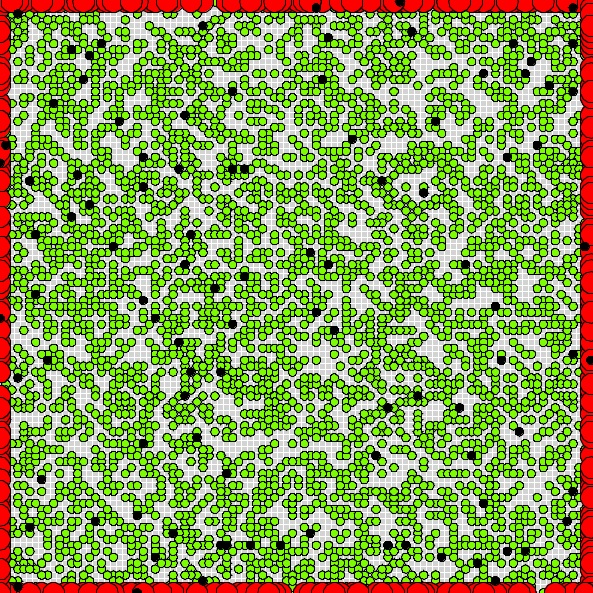
\includegraphics[scale=0.4]{kb2}
\end{center}
\caption{\textit{Hoa (màu đỏ) được phân bố tại biên của thửa ruộng}}
\end{figure}

\begin{figure}
\begin{center}
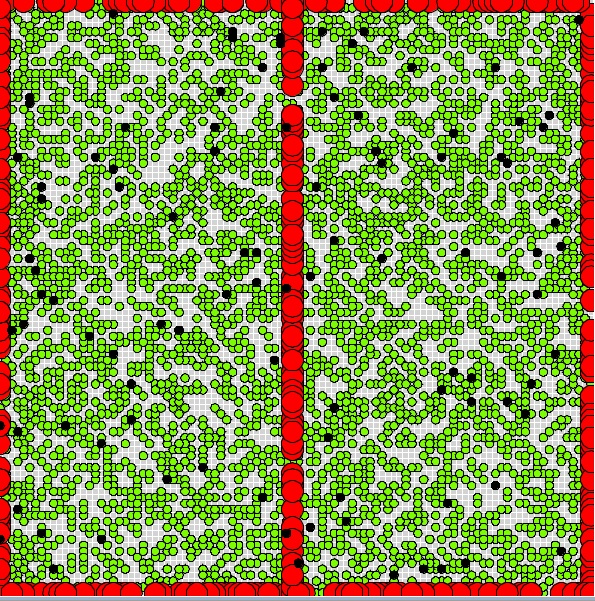
\includegraphics[scale=0.4]{kb3}
\end{center}
\caption{\textit{(Hoa (màu đỏ) được phân bố trên biên và một đoạn thẳng trung tuyến}}
\end{figure}
%h1: Hoa (màu đỏ) được phân bố theo các kịch bản khác nhau trên ruộng

\textit{Thiên địch}: Rầy nâu có một số loài  thiên địch có thể tiêu diệt được và được
ứng dụng như biện pháp sinh học phòng trừ rầy nâu. Cụ thể trong mô hình này, chúng tôi xét thiên địch là loài Nhện ăn thịt (Lycosa  pseudoannulata). Loài nhện này thường gặp rất 
nhiều trên ruộng lúa, chúng chủ động tấn công rầy rất nhanh. Một 
con nhện trưởng thành có thể ăn thịt từ 5-15 con rầy nâu mỗi 
ngày. Ngòai rầy nâu chúng còn tấn công nhiều loài sâu hại khác 
như  bướm của của các loài sâu thuộc Bộ cánh phấn...

\textit{Rầy nâu}: Số lượng rầy nâu $N_3$, rầy nâu được mô phỏng theo vòng đời của chúng. Số lượng rầy nâu thay đổi do tỉ lệ sinh  $r_3$, tỉ lệ chết theo thời gian  $\mu_3$ và sinh trưởng khi chích hút lúa hay bị thiên địch ăn thịt.

Vòng đời của rầy nâu kéo dài khoảng 25-28 ngày ở nhiệt độ $25-30^0C$, bao gồm ba giai đoạn sinh trưởng: trứng, con non và con trưởng thành. Sau khi trứng nở từ 5-7 ngày, con non trải qua năm giai đoạn trong vòng 12-14 ngày và phát triển thành con trưởng thành cánh ngắn hoặc cánh dài. Sự thay đổi sinh học này của rầy nâu tùy thuộc vào điều kiện thời tiết và môi trường từng địa phương [Mochida and Okada, 1979]. Các con trưởng thành cánh ngắn theo quy luật sẽ xuất hiện trước giai đoạn lúa làm đòng và đầu vụ thu hoạch, trong khi con trưởng thành cánh dài phát triển mạnh để di cư. Mỗi lần đẻ trứng, một con rầy cái trưởng thành cánh ngắn có thể sinh 300 trứng và 100 trứng với một con cánh dài trưởng thành [13].

%Nhiệt độ là nhân tố có ảnh hưởng nhất tới sự chuyển giữa giai đoạn sinh trưởng của %rầy nâu [Mochida and Okada, 1979]. Cụ thể được mô tả theo bảng 
Cụ thể, sự phát triển của rầy nâu theo thời gian liên tục tuân theo các phương trình mô tả trong Bảng 3.1. [13]
\begin{table}
\begin{tabular}{m{7cm} m{8cm}}
\hline
{Sự biến đổi} & \textit{Phương trình} \\ 
\hline
\textit{Số lượng trứng} & $E(t+1) = [E(t)-E'(t)+E1(t)]*R_e$ \\ 
\hline
\textit{Số lượng con non} & $N(t+1)=[N(t)-N'(t)+E'(t)*P_e]*R_n$ \\ 
\hline
\textit{Số lượng con trưởng thành} & $MS+ML+FMS+FML$ \\
\hline
\textit{Số lượng con trưởng thành đực cánh ngắn} & $MS(t+1)=[MS(t)-MS'(t)+N'(t)*P_n*S_a]*R_a$ \\
\hline
\textit{Số lượng con trưởng thành đực cánh dài} & $ML(t+1)=[ML(t)-ML'(t)+N'(t)*P_n*S_a]*R_a$ \\
\hline
\textit{Số lượng con trưởng thành cái cánh ngắn} & $FMS(t+1)=[FMS(t)-FMS'(t)+N'(t)*P_n*S_a]*R_a$ \\
\hline
\textit{Số lượng con trưởng thành cái cánh dài} & $FML(t+1)=[FML(t)-FML'(t)+N'(t)*P_n*S_a]*R_a$ \\
\hline
\textit{Số lượng trứng sinh ra (giai đoạn rầy trưởng thành đẻ trứng)} & $E1(t+1)=FMS*300+FML*100$ \\
\hline
\end{tabular}
\caption{\textit{Các hàm biểu thị sự phát triển của rầy nâu theo thời gian liên tục}}
\end{table}
 
{%\eqref{Hình 1}
%h1: Vòng đời rầy nâu và các nhân tố ảnh hưởng
%\begin{figure}%\label{Hình 1}
%\begin{center}
%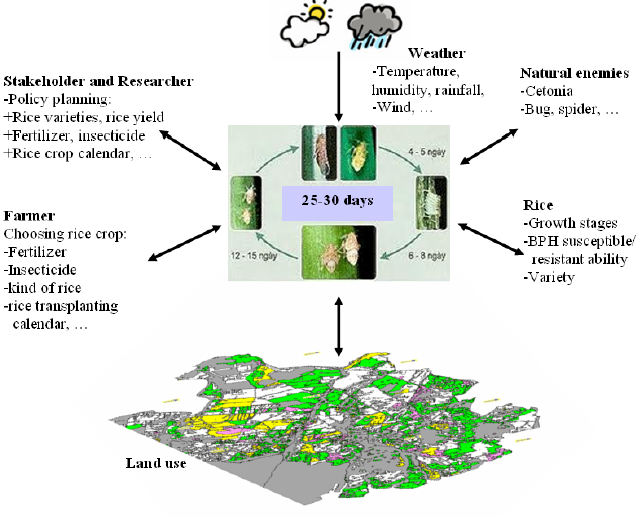
\includegraphics[scale=0.8]{ahg}
%\end{center}
%\caption{\textit{Vòng đời rầy nâu và các nhân tố ảnh hưởng \cite{nngv} }}
%\end{figure}}

\subsection*{Phạm vi}
Phạm vi không gian mô hình xét đến là trên một thửa ruộng. Phạm vi thời gian của mô hình là 120 ngày xét trên thang thời gian sinh trưởng của lúa, đơn vị thời gian là 0.5 ngày nghĩa là mỗi bước mô phỏng tương ứng với 0.5 ngày.

\section{Tiến trình và kế hoạch}

\textit{\indent Cây lúa}: Khi bắt đầu mô phỏng, lượng lúa được phân bố ngẫu nhiên trên ruộng và vị trí cố định cho đến lúc bị chết đi. Lúa sinh trưởng nhờ việc lấy khoáng từ vị trí nó. Lúa khi bước vào giai đoạn đẻ nhánh trong giai đoạn sinh trưởng (đủ tuổi) bắt đầu bị rầy tấn công. Thời điểm thường bắt đầu từ ngày thứ 45 trở đi \cite{sachhd2}. Rầy non cũng có khả năng hút nhựa lúa. Rầy nâu trưởng thành di chuyển theo hướng gió gặp lúa đủ tuổi, nó sẽ chích hút nhựa lúa, khiến lúa chết (xem Hình 3.3).

\textit{Hoa:} Khi bắt đầu mô phỏng, hoa được phân bố theo các kịch bản khác nhau (xem Hình 3.1 - 3.2) và giữ vị trí cố định trong cả quá trình mô phỏng. Hoa sinh trưởng nhờ việc lấy khoáng từ vị trí của nó. Nếu vị trí hoa và lúa nằm trong phạm vi đủ gần, chúng sẽ cạnh tranh khoáng chất với nhau. Rầy nâu trưởng thành di chuyển theo hướng gió nếu gặp thiên địch, khi đó rầy sẽ bị thiên địch ăn thịt, một phần xác rầy chết rơi xung quanh cây hoa và làm nguồn dinh dưỡng cho cây.

\textit{Thiên địch:} Thiên địch bị thu hút đến vùng có hoa, số lượng thiên địch sẽ tăng theo mỗi bước thời gian. Xét với loài nhện ăn thịt, chúng có vòng đời 30 ngày tương tự như rầy nâu. Khả năng sinh sản mỗi lần của một con nhện cái cũng có thể tới 300 trứng.

\textit{Rầy nâu:} Rầy nâu là loài côn trùng có chu kì phát triển theo kiểu biến thái không hoàn toàn, phải trải qua 3 pha phát dục: pha trứng, pha ấu trùng (rầy non) và pha trưởng thành. Vòng đời phát triển của rầy nâu được mô tả trong Hình 2.6. Trong điều kiện nhiệt độ $25-30^o C$, vòng đời rầy nâu thường từ 25-30 ngày: trứng phát triển thành rầy non từ 5-7 ngày, rầy non trưởng thành từ 12-14 ngày, sau đó đẻ trứng và chết đi \cite{sachhd1}. Rầy trưởng thành có hai loại: cánh dài và cánh ngắn. Rầy trưởng thành cánh dài xâm nhập vào ruộng lúa và đẻ trứng trên các bẹ lá hoặc ở các gân lá \cite{sachhd2}. Rầy non có màu trắng, các tuổi sau có màu vàng nâu \cite{sachhd2}. Rầy cánh dài thường xuất hiện vào giai đoạn đầu và giai đoạn lúa chín, di chuyển, phát tán. Rầy trưởng thành di chuyển 0.5 ngày/ lần. Phòng thí nghiệm Viện Khoa Học Kĩ Thuật Nông Nghiệp Miền Nam cho số liệu một trưởng thành cái của rầy nâu đẻ trung bình 150-400 trứng. Nuôi thí nghiệm ở Long An, mỗi trưởng thành cái đẻ 50-200 trứng. Tronh điều kiện vùng Hà Nội, một trưởng thành cái có khả năng đẻ 110 - 324 trứng \cite{sachhd1}.

%hình 3
\begin{figure}
\begin{center}
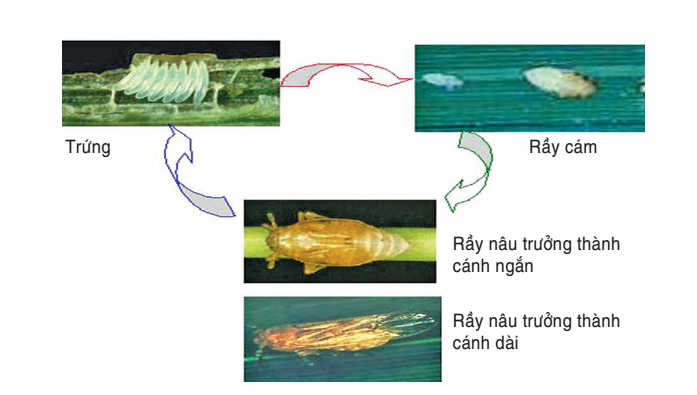
\includegraphics[scale=0.8]{vongdoiray}
\end{center}
\caption{\textit{Vòng đời phát triển của rầy nâu}}
\end{figure}

\textit{Lịch trình:} Khi bắt đầu mô phỏng, lúa và rầy được phân bố ngẫu nhiên trên các ô khoáng, hoa được phân bố ngẫu nhiên hay theo cách sắp xếp với số lượng ban đầu cụ thể. Tai mỗi bước thời gian của mô phỏng, lúa và hoa sinh trưởng nhờ việc lấy khoáng từ ô khoáng chất tại vị trí của chúng, đồng thời age của lúa, hoa và rầy đều tăng lên và energy của chúng mất đi một lượng cho sinh trưởng. Đến ngày 21, rầy trưởng thành và bắt đầu đẻ trứng và 7 ngày sau kết thúc vòng đời đầu tiên. Rầy sẽ lặp lại vòng đời theo chu kì 30 ngày. Đến ngày 45, lúa bước vào giai đoạn đẻ nhánh và bắt đầu bị rầy tấn công. Rầy trưởng thành di chuyển theo tốc độ và hướng gió, khi gặp và hút nhựa lúa khiến lúa chết. Nếu rầy di chuyển gặp hoa, nó sẽ bị thiên địch ăn thịt.

\section{Các khái niệm nền tảng}
\subsection{Các quy tắc cơ bản}
\indent Rầy di chuyển theo gió gặp lúa và hại lúa có thể theo cách trực tiếp là chích hút nhựa lúa hoặc gián tiếp môi giới truyền vi rút gây bệnh vàng lùn, lùn xoắn lá cho cây lúa. Cả hai cách đều khiến lúa không trổ bông được, năng suất giảm nghiêm trọng hay mất trắng \cite{tltk9, tltk10}.

\indent Rầy hút được nhựa lúa biến thành năng lượng để sống. Tuy nhiên, nếu rầy di chuyển tới vùng có hoa, gặp thiên địch, nó sẽ bị thiên địch ăn thịt và một phần xác rơi xuống làm dưỡng chất cho hoa.

\indent Các thực thể trong mô hình là lúa, hoa, thiên địch và rầy mất năng lượng theo từng bước thời gian do sinh trưởng ngoài ra còn mất năng lượng do di chuyển (thiên địch và rầy nâu).

\subsection{Sự nổi bật}
Sự nổi bật hay kết quả đầu ra ta quan tâm nhất ở đây là ảnh hưởng của phân bố không gian của hoa trên ruộng tới sự sinh trưởng và hại lúa của rầy nâu, điều chưa đoán biết được trong các điều kiện đầu vào ban đầu của mô hình và sự thay đổi của môi trường.

\subsection{Mục tiêu}
Mục tiêu của mô hình là xem xét sự khác nhau của mật độ sinh trưởng và hại lúa của rầy nâu cùng với sự phát triển của lúa với những kịch bản phân bố vị trí không gian của hoa khác nhau trên ruộng lúa (Hình 3.1 - 3.2). Mục tiêu này được rút ra từ việc ghi nhận sự phát triển về số lượng rầy nâu cũng như số lượng phát triển của lúa theo thời gian.

\subsection{Tương tác}
Tương tác giữa rầy và lúa là việc rầy hút nhựa lúa, khiến lúa chết, ảnh hưởng tới năng suất. Hoa thu hút thiên địch của rầy tới vùng có trồng hoa, nên rầy sẽ bị thiên địch ăn thịt khi di chuyển tới vùng có hoa, ảnh hưởng tới mật độ rầy. Đồng thời, vùng hoa sẽ cản bước di chuyển của rầy. Lúa và hoa có tương tác cạnh tranh khoáng trong đất để sinh trưởng.

\subsection{Quan sát}
Chúng tôi ghi nhận số lượng rầy nâu và lúa trên ruộng trước và sau mỗi ngày. Từ đó thu được số liệu về mật độ rầy và số lúa chết mỗi ngày.

\section{Khởi tạo}
khởi tạo mô phỏng với 300000 cây lúa, 300 con rầy được phân bố ngẫu nhiên trên ruộng. 1000 cây hoa cũng được khởi tạo khi bắt đầu mô phỏng và được phân bố tương ứng với 2 kịch bản phân bố không gian: (a) Hoa phân bố tại biên của thửa ruộng (b) Hoa phân bố trên biên và một đoạn thẳng trung tuyến (Hình 3.1 - 3.2).

\section{Dữ liệu đầu vào}
Trạng thái rầy di chuyển được mô phỏng phụ thuộc vào hướng và tốc độ gió, là các điều kiện môi trường cần dữ liệu đầu vào.

\section{Mô hình con}
\textit{Rầy hại lúa:} Rầy ở giai đoạn con non cũng đã có khả năng hút nhựa khiến lúa mất đạm, khô mà chết. Rầy hại lúa khi nó bước vào giai đoạn trưởng thành (có thể di chuyển) và lúa vào giai đoạn đẻ nhánh (đủ tuổi) không chỉ hút đạm mà còn thêm khả năng truyền virut gây bệnh (vàng lùn, lùn xoắn lá,...).

\textit{Hoa ăn rầy:} Khi di chuyển, nếu rầy theo hướng gió di chuyển tới vị trí vùng có hoa, nếu gặp thiên địch, rầy sẽ bị ăn thịt.

\textit{Sự cạnh tranh khoáng chất:} Lúa và hoa cạnh tranh khoáng tại vị trí của mình để sinh trưởng.

Từ đó, chúng tôi đề xuất mô hình phương trình (Equation-based model viết tắt là EBM) thể hiện sự thay đổi mật độ các loài trong mô hình dựa trên cá thể (Agent-based model viết tắt là ABM) đang xét

\begin{flushleft}
\begin{equation}\label{1}
\dfrac{d N_1}{dt} = r_1 N_1 - \mu_1 N_1 - a_{12} N_1  N_2 - b_{31} N_1 N_3
\end{equation}
\begin{equation}\label{2}
\dfrac{d N_2}{dt} = r_2 N_2 - \mu_2  N_2 - a_{21} N_2 N_1 + b_{23} e_{23} N_2 N_3
\end{equation}
\begin{equation}\label{3}
\dfrac{d N_3}{dt} = r_3 N_3 - \mu_3  N_3 + b_{31} e_{31} N_3 N_1 - b_{23} N_2 N_3
\end{equation}
\end{flushleft}

\indent(1) Lúa sinh trưởng tự nhiên với tỉ lệ sinh $r_1$, bị chết theo tỉ lệ chết $\mu_1$, cạnh tranh khoáng với hoa theo hệ số cạnh tranh $a_{12}$  và chết do bị rầy ăn với hệ số bắt mồi $b_{31}$.

(2) Hoa sinh trưởng tự nhiên với tỉ lệ sinh $r_2$, bị chết theo tỉ lệ chết $\mu_2$, sinh trưởng nhờ xác rầy chết theo tỉ lệ chuyển hóa $b_{23} e_{23}$ và cạnh tranh khoáng với hoa theo hệ số cạnh tranh $a_{21}$.

(3) Rầy nâu sinh trưởng tự nhiên với tỉ lệ sinh $r_3$, bị chết theo tỉ lệ chết $\mu_3$, sinh trưởng nhờ thức ăn ăn được từ lúa theo tỉ lệ chuyển hóa $b_{31} e_{31}$ và chết do bị hoa ăn với hệ số bắt mồi $b_{23}$.

\section*{Kết luận}
Trong chương 3, chúng tôi đã mô tả mô hình đa tác tử của rầy nâu và lúa với phân bố hoa thu hút thiên địch của rầy theo giao thức chuẩn ODD. Với các trạng thái và hành vi của các thực thể trong mô hình đã được mô tả, chúng tôi thực hiện xây dựng chương trình mô phỏng cho mô hình đang xét bằng phần mềm GAMA. Trong chương 4, chúng tôi sẽ trình bày việc xây dựng chương trình mô phỏng của mô hình và các kết quả thu được từ chương trình mô phỏng.

\newpage
\chapter{Kết quả nghiên cứu và thảo luận}
\section{Các thí nghiệm mô phỏng}
\subsection{Thí nghiệm 1}
Mô phỏng được xây dựng trong môi trường grid phạm vi $ 100 \times 100$. Khởi tạo mô phỏng với 30000 cây lúa, 1000 cây hoa, 700 con nhện (thiên địch) và 300 con rầy.

Mỗi cây lúa được mô phỏng như một cá thể của loài lúa, gồm các thuộc tính:
\begin{itemize}
\item location: ô vị trí sinh trưởng, cố định trong suốt quá trình mô phỏng.
\item energy: năng lượng nội tại, cây lúa chết khi energy <=0.
\item age: tuổi lúa, sử dụng để xác định thời điểm mà lúa bắt đầu bị rầy tấn công.
\end{itemize}

Mỗi cây hoa được mô phỏng như một cá thể của loài hoa, gồm các thuộc tính:
\begin{itemize}
\item location: ô vị trí sinh trưởng, cố định trong suốt quá trình mô phỏng.
\item energy: năng lượng nội tại, cây hoa cũng chết khi energy <=0.
\end{itemize}

Mỗi con nhện được mô phỏng như một cá thể của loài thiên địch, gồm các thuộc tính:
\begin{itemize}
\item location: ô xác định vị trí cá thể.
\item energy: năng lượng nội tại của cá thể, nhện chết khi energy <=0. Năng lượng của nhện tăng lên nếu nó bắt và ăn thịt được rầy.
\item age: tuổi nhện, sử dụng để xác định giai đoạn vòng đời sinh trưởng của nhện.
\end{itemize}

Mỗi con rầy được mô phỏng như một cá thể của loài rầy, gồm các thuộc tính:
\begin{itemize}
\item location: ô vị trí rầy
\item energy: năng lượng nội tại của cá thể rầy, rầy chết khi energy <=0. Năng lượng của rầy tăng lên nếu nó di chuyển đến vị trí có lúa và ăn lúa, khiến lúa chết.
\item age: tuổi rầy, sử dụng để xác định rầy thuộc pha nào trong vòng đời sinh trưởng.
\end{itemize}

Chương trình mô phỏng dưới dạng giải thuật sau:

\textit{\textbf{Đầu vào:}} Dữ liệu đầu vào về thời tiết: hướng, vận tốc gió; Số lượng các loài ban đầu; Tham số hành vi của từng loài: tỉ lệ chuyển hóa, năng lượng sinh sản, năng lượng mất do sinh trưởng.

\textbf{\textit{Đầu ra:}} Đồ thị thể hiện số lượng các loài biến đổi trong mô hình theo mỗi bước mô phỏng.
%\Khung{.9\textwidth}{
\begin{center}
\small{
\begin{verbatim}
foreach time_step from 1 to time=120#day do
	foreach agent is in [lua] do
	update lua age;
	foreach agent is in [ray] do
	update  age;
	if age>=30 then do die;
	if age>=7 then
	get wind_dir, wind_speed of current time step;
	do wind_move and eat_rice;
	if age >=21 then do reproduce;
	foreach agent is in [thien_dich]
	update hoa location
	do migrate and eat_ray;
\end{verbatim}
}
\end{center}

Quá trình mô phỏng được chạy với các giá trị ban đầu khởi tạo của các loài như nhau, chương trình chạy 50 lần mô phỏng để lấy số liệu phát triển của ba loài xét trong mô hinh trung bình tương ứng với mỗi kịch bản (a) Hoa phân bố tại biên của thửa ruộng (b) Hoa phân bố trên biên và một đoạn thẳng trung tuyến. Hình 4.1 và Hình 4.2 mô tả đồ thị theo thời gian của các loài tương ứng với mỗi kịch bản. Hình 4.3 là đồ thị biểu diễn sự phát triển của rầy với các kịch bản đang xét trong một trường hợp chạy mô phỏng.

\begin{figure}%\label{Hình 1}
\begin{center}
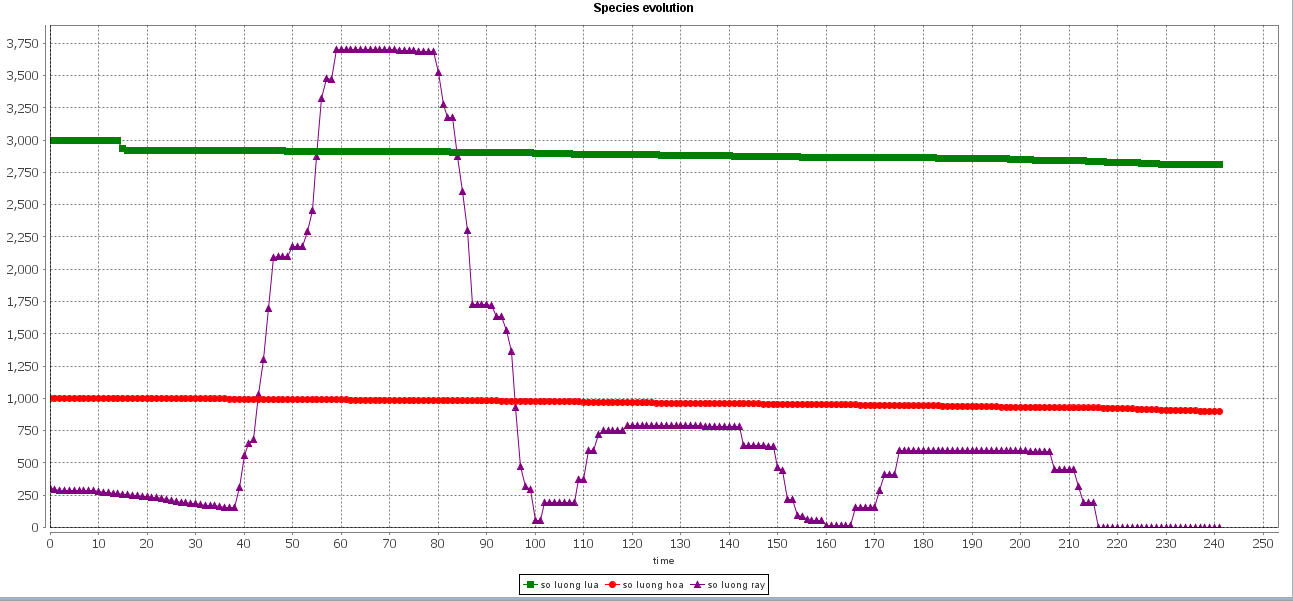
\includegraphics[scale=0.4]{kb2gr}
\end{center}
\caption{\textit{Sự phát triển của các loài theo thời gian trong một lần chạy mô phỏng (kịch bản (a))}}
\end{figure}

\begin{figure}%\label{Hình 1}
\begin{center}
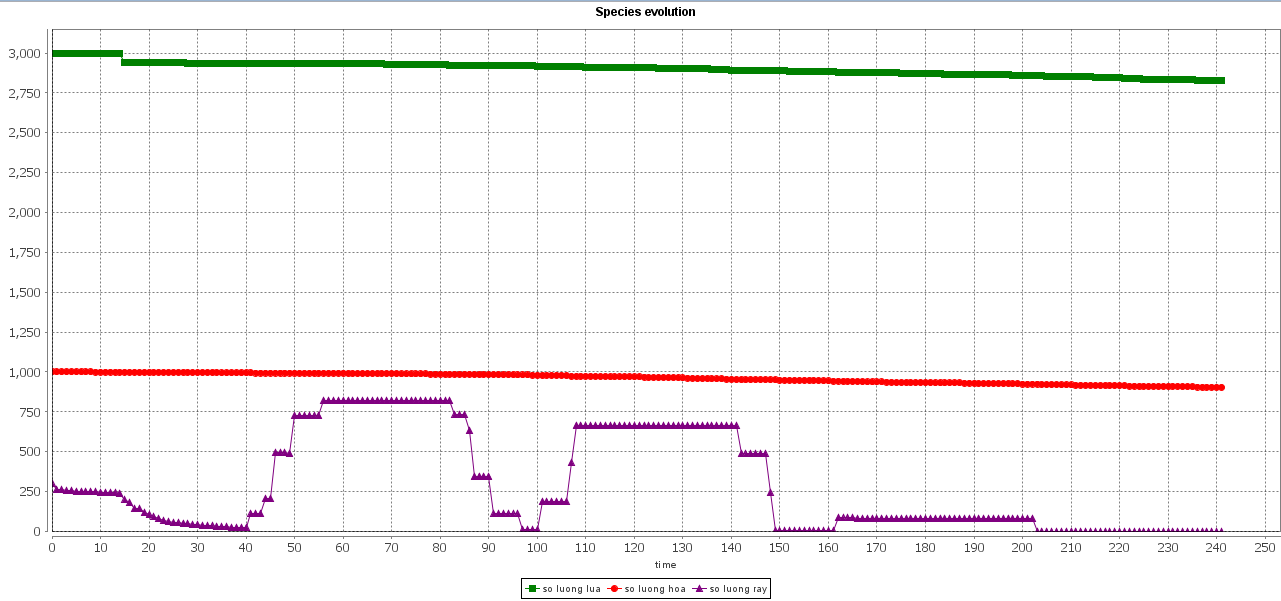
\includegraphics[scale=0.4]{kb3gr}
\end{center}
\caption{\textit{Sự phát triển của các loài theo thời gian trong một lần chạy mô phỏng (kịch bản (b)}) }
\end{figure}

\begin{figure}%\label{Hình 1}
\begin{center}
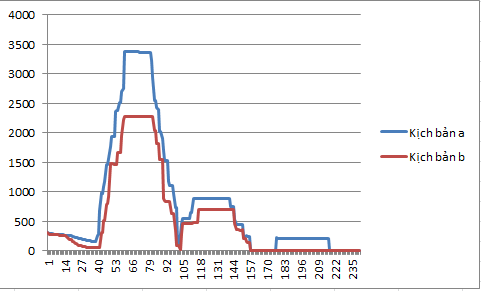
\includegraphics[scale=1]{2kb}
\end{center}
\caption{\small Sự phát triển của rầy theo thang thời gian tương ứng với hai kịch bản }
\end{figure}

\subsection{Thí nghiệm 2}
Mở rộng mô hình với hai kịch bản xét trên 9 thửa ruộng (xem Hình 4.4 - 4.5). Khởi tạo mô phỏng với 30000 cây lúa, 1000 cây hoa, 700 con nhện (thiên địch) ở mỗi thửa ruộng. Khởi tạo 300 con rầy ban đầu chỉ tại thửa ruộng thứ nhất.
\begin{figure}%\label{Hình 1}
\begin{minipage}[b]{0.5\linewidth}
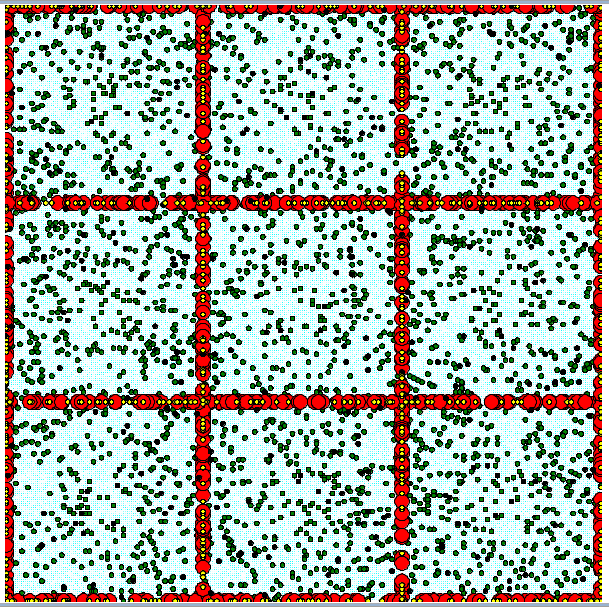
\includegraphics[scale=0.4]{kb91}
\caption{\textit{ Mô phỏng mở rộng trên 9 thửa ruộng tương ứng với kịch bản (a)}}
\end{minipage}
\hspace{0.5cm}
\begin{minipage}[b]{0.5\linewidth}
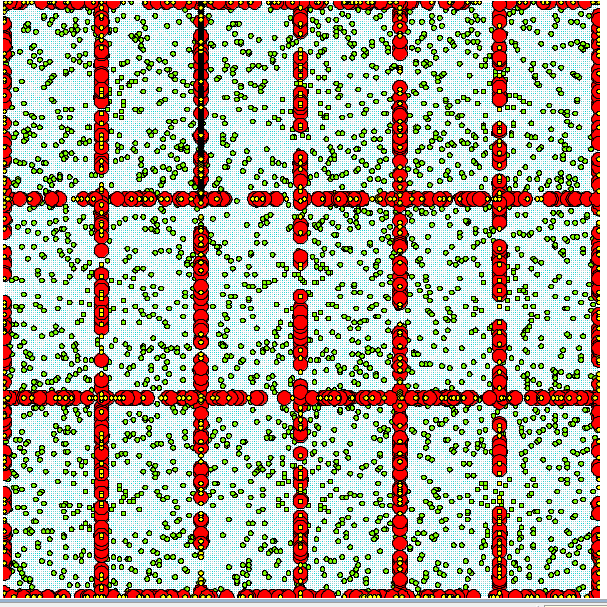
\includegraphics[scale=0.4]{kb92}
\caption{ \textit{Mô phỏng mở rộng trên 9 thửa ruộng tương ứng với kịch bản (b)} }
\end{minipage}
\end{figure}


\begin{figure}%\label{Hình 1}
\begin{center}
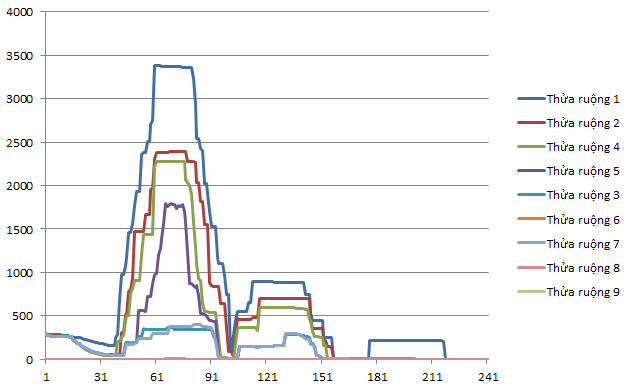
\includegraphics[scale=0.8]{kq9a}
\end{center}
\caption{ \textit{Số lượng rầy nâu trên 9 thửa ruộng tương ứng với kịch bản (a)}}
\end{figure}

\begin{figure}%\label{Hình 1}
\begin{center}
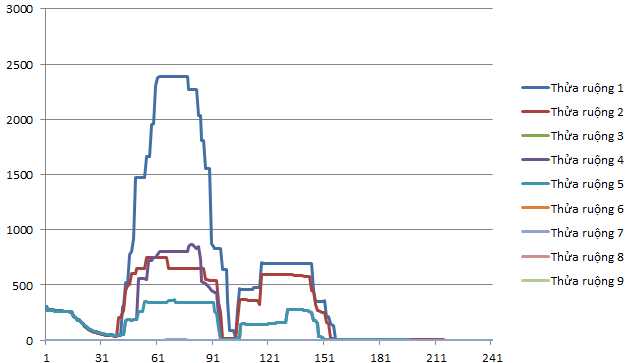
\includegraphics[scale=0.8]{kq9b}
\end{center}
\caption{\textit{Số lượng rầy nâu trên 9 thửa ruộng tương ứng với kịch bản (b)} }
\end{figure}

%\begin{figure}%\label{Hình 1}
%\begin{center}
%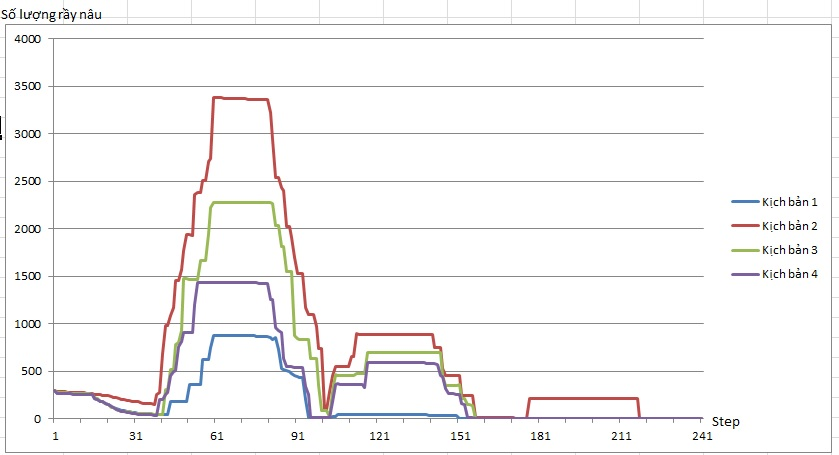
\includegraphics[scale=0.6]{4kbrn}
%\end{center}
%\caption{\small Sự phát triển của rầy theo thang thời gian tương ứng tăng lượng rầy ban đầu }
%\end{figure}
%Mở rộng mô hình xét trên 9 thửa ruộng, với cùng lượng rầy ban đầu chỉ trong một thửa, kết quả trung bình đạt được như sau.\\


\section{Các kết quả đạt được}
Từ đồ thị, tôi đưa ra so sánh lượng rầy phát triển trong cả quá trình mô phỏng giữa hai kịch bản như sau: Mật độ rầy giảm đi trong kịch bản (b) so với kịch bản (a). Việc phân bố hoa theo cả đường biên và đường trung tuyến có kết quả hạn chế sự phát triển rầy nâu tốt hơn so với việc chỉ phân bố hoa trên biên.
%Mật độ hoa trên ruộng cũng có ảnh hưởng đến sự phát triển của rầy. Cụ thể, số liệu được thể hiện trong Hình 3.4 và Hình 3.5. Trong cả hai kịch bản, khi số lượng hoa tăng, lượng rầy có thay đổi theo chiều hướng giảm.

Với trường hợp mở rộng mô hình xét trên 9 thửa ruộng, với cùng lượng rầy ban đầu chỉ trong một thửa, trường hợp trồng hoa trên biên và một đường trung tuyến vẫn cho kết quả ngăn chặn sự phát triển của rầy tốt hơn. Hơn thế nữa, việc trồng hoa trên biên và đường trung tuyến còn có tác dụng ngăn cản bước di chuyển của rầy. Kịch bản (a) mở rộng với phạm vi 9 thửa ruộng, rầy lây lan qua phạm vi 6 thửa (xem Hình 4.6). Kịch bản (b) mở rộng cho kết quả tốt hơn, rầy hầu như lây lan chỉ qua phạm vi đến 4 thửa là đã bị ngăn chặn hoàn toàn (xem Hình 4.7). 
\newpage

\chapter{Kết luận}
Trong đồ án này, chúng tôi đã giới thiệu và trình bày một số khái niệm cơ bản về mô hình, chu trình phát triển mô hình và mô hình hóa dựa trên cá thể. Chúng tôi cũng giới thiệu tổng quan về giao thức ODD và sử dụng nó để mô tả và xây dựng mô hình rầy nâu hại lúa, từ đó đưa ra kết luận ảnh hưởng phân bố không gian của hoa thu hút thiên địch lên sự phát triển của rầy nâu ứng với hai kịch bản. Các kết quả thu được của đồ án:
\begin{itemize}
\item Xây dựng và mô hình hóa dựa trên cá thể mô hình rầy nâu hại lúa.
\item Mô phỏng sự phát triển và lây lan của rầy nâu ứng với hai kịch bản phân bố không gian của hoa thu hút thiên địch rầy nâu trên GAMA.
\item So sánh sự phát triển của rầy nâu trên ruộng giữa hai kịch bản phân bố không gian của hoa.
\item Kết luận về mối liên hệ giữa phân bố không gian của hoa với sự phát triển và lây lan của rầy nâu: Xét trên một thửa ruộng và mô hình mở rộng với 9 thửa ruộng, việc trồng hoa theo đường biên và một trung tuyến có kết quả diệt và ngăn chặn rầy tốt hơn so với chỉ trồng trên biên với cùng số lượng hoa đó
\end{itemize} 

Hướng phát triển tiếp theo chúng tôi muốn mở rộng mô phỏng trong không gian lớn với số lượng cá thể lúa, hoa, rầy tới vài trăm triệu cá thể trên nhiều thửa ruộng của một xã, huyện thậm chí là một vài tỉnh để từ đó giúp người nông dân đưa ra quyết định tốt hơn trong việc diệt trừ rầy nâu hại lúa. Hơn nữa, chúng tôi sẽ áp dụng mô hình trên môi trường thực tế dựa vào bản đồ thông tin địa lý (Geographic Information system viết tắt là \textit{GIS}) của các vùng trồng lúa ở Việt Nam.\\
\newpage
\addcontentsline{toc}{chapter}{{Danh mục công trình công bố của tác giả}}
\chapter*{Danh mục công trình công bố của tác giả}
\begin{flushleft}
\quad $[1]$\ Vũ Thu Thảo, Nguyễn Ngọc Doanh, Nguyễn Nhị Gia Vinh, Nguyễn Thị\\\quad \quad \   Ngọc
Anh, \textit{"Mô hình hóa ảnh hưởng phân bố không gian của hoa diệt rầy\\ \quad \quad \  tới
sự phát triển của rầy nâu hại lúa"}, Tạp chí Khoa học và Công nghệ -\\\quad \quad \  Đại học Thái Nguyên, 2015, pp.119-123.\\
\end{flushleft}
\newpage
\addcontentsline{toc}{chapter}{{Tài liệu tham khảo}}
\bibliographystyle{amsplain}
\thispagestyle{empty}
\bibliography{science}
\end{document}